\chapter{LLM-Based Reasoning for Open-Set Modulation Classification: Plug-and-Play and DiSC-AMC}
\label{chap:plugandplay}


\section{Introduction}
\IEEEPARstart{A}{utomatic} Modulation Classification (AMC) is a critical technology in modern wireless communications, underpinning applications in cognitive radio, spectrum sensing, and interference management. By accurately identifying modulation schemes, AMC facilitates efficient spectrum utilization and enhances the adaptability and reliability of communication networks. However, despite its significance, AMC remains a challenging problem due to the complex interplay of signals with ambient noise and other channel impairments.

Early approaches to AMC predominantly relied on traditional machine learning techniques and handcrafted feature extraction, but these methods have gradually been superseded by deep learning models. For instance, Convolutional Neural Networks (CNNs) have been extensively applied in this domain. Peng et al.~\cite{peng2017modulation} transformed raw modulated signals into constellation diagrams to serve as inputs for CNN architectures such as AlexNet, while subsequent studies introduced variants like MCNet~\cite{8963964} that leveraged multiple convolutional blocks with skip connections and asymmetric kernels to capture spatio-temporal correlations. In another investigation, a CNN framework was explored using multiple signal representations, such as constellation diagrams, ambiguity functions, and eye diagrams, with empirical results indicating that combining these representations could improve classification accuracy~\cite{10139474}.

\begin{figure*}
    \centering
    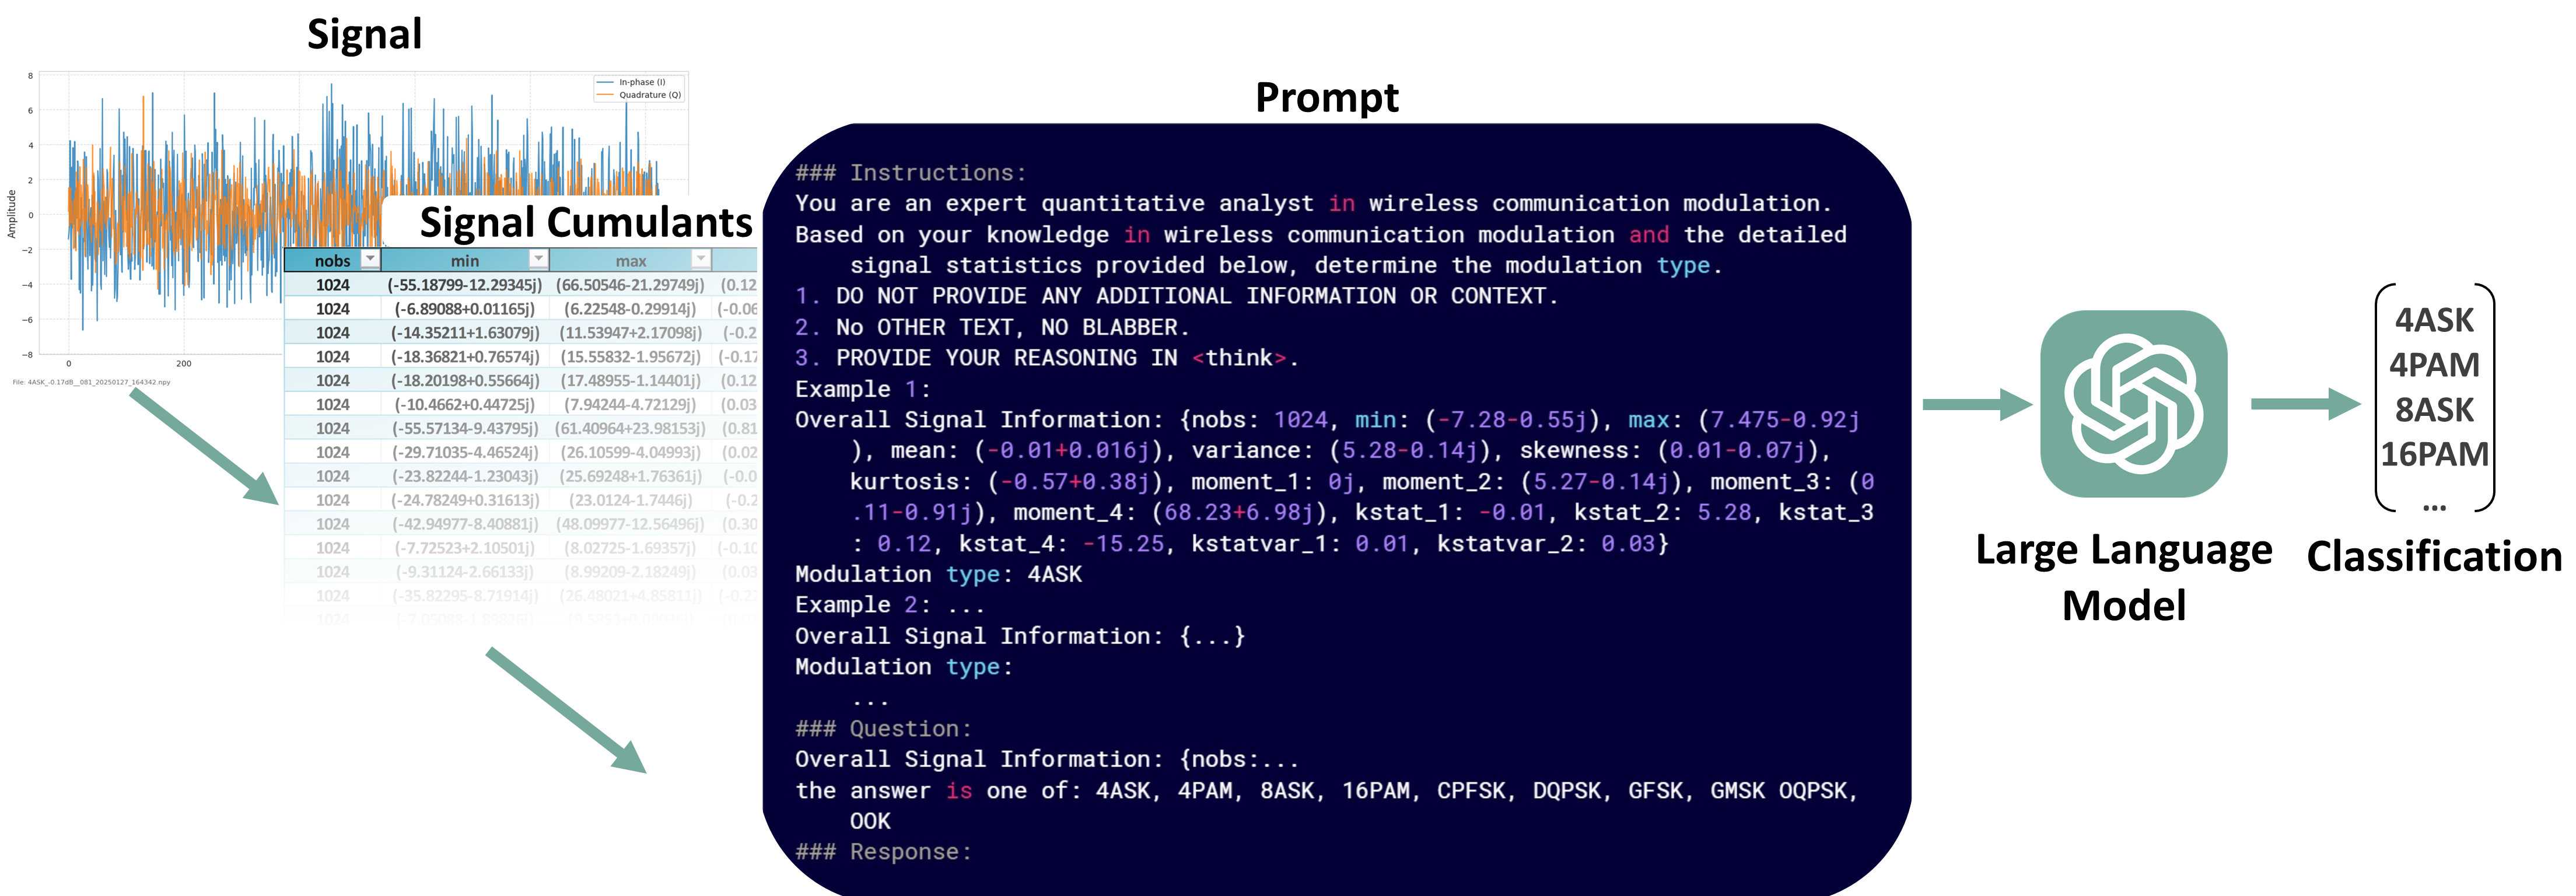
\includegraphics[width=0.9\textwidth]{FIGURES/pnp/method.png}
    \caption{Overview of our in-context AMC framework. The raw signal is first summarized into high-order statistics and cumulants, which are then embedded in a text prompt. This prompt is fed into a large language model to perform modulation classification from a predefined set of modulation types (e.g., 4ASK, 4PAM, 8ASK, 16PAM).}
    \label{fig:method}
\end{figure*}

More recently, attention-based models, particularly transformers, have garnered significant interest for AMC. Transformers, introduced by Vaswani et al.~\cite{vaswani2017attention}, are adept at processing sequential data by dynamically focusing on the most relevant parts of the input. Cai et al.~\cite{cai2022signal} demonstrated that a transformer network (TRN)-based approach can capture long-range dependencies more effectively than conventional CNNs, which is especially beneficial in low SNR scenarios. Building on this idea, Kong et al.~\cite{kong2023transformer} further improved transformer-based AMC by incorporating convolutional embedding and attention pooling techniques, and Qu et al.~\cite{qu2024enhancing} combined transformers with Long Short-Term Memory (LSTM) networks to address long-range temporal dependencies and enhance robustness against noise through novel data augmentation strategies.

Despite these advancements, many existing methods are developed under idealized, noise-free conditions~\cite{peng2018modulation,8454504}. Such conditions are rarely encountered in real-world environments where signals are typically contaminated with noise. Moreover, several approaches struggle with fine-tuning downstream tasks when only limited labeled data is available~\cite{hong2017automatic,ramjee2019fast}.

Nmformer \cite{faysal2024nmformer} employs a Vision Transformer (ViT) trained on a large labeled dataset to achieve strong performance when retrained on low-SNR signals. However, the model struggles to attain high accuracy due to the absence of unsupervised pretraining. In contrast, DenoMAE \cite{faysal2025denomae} and DenoMAE2.0 \cite{faysal2025denomae20improvingdenoisingmasked} aim to achieve competitive performance with only a few thousand samples during pretraining and significantly fewer labeled samples in the downstream task. Nevertheless, the limited data constrains the model's ability to achieve substantial performance improvements. This underscores the need for a more advanced framework that effectively leverages large-scale data to enhance accuracy.

Addressing these limitations, recent work has begun to explore more sophisticated frameworks that can balance performance across varying SNR conditions. Gao et al. in the MoE-AMC study~\cite{gao2023moe} proposed a Mixture-of-Experts (MoE) approach that integrates a ResNet-based model for high SNR signals with a transformer-based model for low SNR signals, achieving a more balanced and robust classification performance. Complementing this, the review by Jafarigol et al.~\cite{jafarigol2025ai} provided a comprehensive analysis of contemporary AI/ML-based AMC models, highlighting both recent advances and persistent challenges, particularly the difficulty of maintaining accuracy in noisy environments and the need for efficient models that operate under constrained computational resources.

In this work, we take a novel direction by leveraging a pretrained LLM-based approach for automatic modulation classification. Our method utilizes traditional modulation statistics and cumulants, capitalizing on the LLM’s inherent familiarity with classical signal processing techniques. This capability enables our framework to perform competitive one-shot modulation classification without the need for exhaustive training across all SNRs, modulation types, or channel conditions, and without the computational overhead of extra preprocessing steps such as denoising. By transforming quantitative signal features into natural language descriptions, our approach bridges the gap between classical signal processing and modern AI, achieving robust performance even in challenging, noisy scenarios.

Our contributions include:
\begin{itemize}
    \item A novel in-context approach for AMC using LLMs that simplifies the processing pipeline.
    \item A one-shot classification method that eliminates the need for extensive training data.
    \item Competitive performance under both noiseless and noisy conditions.
\end{itemize}

\textbf{Framework Position:} Within the dissertation's modular framework for Wireless Physical-Layer Foundation Models (WPFMs), this Plug-and-Play approach serves as the \textit{intelligent reasoning engine}—the second core component. While DenoMAE (Chapter~\ref{chap:denomae}) learns rich signal representations through self-supervised learning and Meta-Task (Chapter~\ref{chap:meta_task}) enables rapid adaptation with minimal data, Plug-and-Play demonstrates a fundamentally different pathway: leveraging pre-trained LLMs to perform training-free wireless classification by converting statistical signal features into natural language prompts. This validates the dissertation's central thesis that wireless foundation models need not be built through massive isolated training but can strategically approximate and integrate world knowledge. By achieving competitive performance (72.4\% accuracy) without wireless-specific training, this work proves that sophisticated reasoning capabilities can be transferred from language models to the wireless domain, providing interpretability, open-set classification, and cost-effective deployment. The modular design enables future integration where DenoMAE's learned features could replace or augment the statistical summaries, while Meta-Task could enable few-shot adaptation of prompt strategies.

Beyond improving AMC performance, our approach paves the way for developing foundation models for wireless communications. Such foundation models can provide a robust unified solution across diverse scenarios, reducing the need for channel-specific models and lowering the associated development and deployment costs. By enabling models that generalize well without extensive retraining, our method has the potential to streamline the design of wireless communication systems, making them more adaptable, scalable, and cost-effective.

Overall, this work not only simplifies modulation classification but also sets the stage for further research in robust, scalable, and versatile signal processing using large language models.

% The remainder of the paper is organized as follows. Section~\ref{sec:back} presents the theoretical background, with an emphasis on high-order cumulants and their application in feature extraction. Section~\ref{sec:meth} details our proposed method and the process of prompt creation for our LLM-based approach. In Section~\ref{sec:exp}, we report experimental results obtained on multiple datasets, and Section~\ref{sec:con} concludes the paper with a discussion of future research directions.

\section{Theoretical Background}
\label{sec:back}

Plug-and-Play rests on classical statistical features of the received signal. The central moments of a signal summarize the shape of its amplitude distribution, and $k$-statistics are the minimum-variance unbiased estimators of its cumulants. Cumulants of order higher than two vanish for Gaussian noise, so they suppress additive Gaussian noise while retaining structure that depends on the modulation, and fourth-order cumulants in particular take different values for BPSK, QPSK, and QAM constellations~\cite{swami2000hierarchical}. These features are compact and interpretable, which is why classical feature-based AMC used them, and they can be written as short numeric descriptions that a language model can read as text.

\section{Method}
\label{sec:meth}
\textbf{Modular Design:} This method operates as a standalone component using statistical signal features, demonstrating training-free classification. Future work could integrate DenoMAE's learned representations (Chapter~\ref{chap:denomae}) as enhanced feature inputs while maintaining the framework's modularity.

In this section, we present a novel approach for modulation classification using higher-order statistics and prompt-based LLM generation through three key stages:

\textbf{(Stage 1)} extracting comprehensive statistical summaries (e.g., moments, variance, kurtosis); \textbf{(Stage 2)} linearizing these features into a text format \cite{wang2023meditab} as
\begin{equation} \text{linearize}(x) = {[c_{k}: x_{k}]}_{k=1}^{K}, \end{equation}
where $c_k$ is the $k^{\mathrm{th}}$ feature name and $x_k$ its value; and \textbf{(Stage 3)} constructing a structured prompt combining instructions ($I$), exemplar context ($C$), the linearized statistics, and modulation directives ($S$):
\begin{equation} d = \text{LLM}\bigl(I, C,\ \text{linearize}(x),\ S\bigr). \end{equation}
This process generates concise signal descriptions to guide the LLM in selecting the appropriate modulation type (Figure~\ref{fig:method}).


\subsection{Signal Summarization}
We compute key descriptive statistics and cumulant-related metrics to obtain a robust statistical characterization of each signal. These statistical summaries serve as the foundation for both individual signal queries and for constructing exemplar contexts, reference points with known modulation labels that help the model infer the underlying patterns associated with each modulation type. Algorithm~\ref{alg:summary} details the procedure used to convert a raw signal vector $x$ into a succinct string $d$ that encapsulates its statistical properties.

\begin{algorithm}
    \caption{Signal Summarization}\label{alg:summary}
    \KwIn{\texttt{$x$} (Vector of signal values)}
    \KwOut{\texttt{$d$} (A string summarizing cumulants and descriptive statistics)}
    
    \small % Optional: reduces font size for the algorithm
    
    % Compute descriptive statistics
    \BlankLine
    \texttt{stats} $\gets$ \{ \\
    \quad \texttt{"nobs"}: $x$.\texttt{nobs},\\
    \quad \texttt{"min"}: $x$.\texttt{min},\\
    \quad \texttt{"max"}: $x$.\texttt{max},\\
    \quad \texttt{"mean"}: $x$.\texttt{mean},\\
    \quad \texttt{"variance"}: $x$.\texttt{variance},\\
    \quad \texttt{"skewness"}: $x$.\texttt{skewness},\\
    \quad \texttt{"kurtosis"}: $x$.\texttt{kurtosis} \\
    \}\;
    \BlankLine
    
    % Compute higher-order moments\\
    \texttt{\# Compute k-th moment and cumulant} \\
    \For{$i \gets 0$ \KwTo $7$}{
        \texttt{stats["moment\_$i$"]} $\gets$ \texttt{moment(signal, order = $i$)}\;
    }
    \BlankLine
    
    % Compute k-statistics
    \For{$i \gets 1$ \KwTo $4$}{
        \texttt{stats["kstat\_$i$"]} $\gets$ \texttt{kstat(signal, $i$)}\;
    }
    \BlankLine
    
    % Compute k-statistic variances
    \For{$i \gets 1$ \KwTo $2$}{
        \texttt{stats["kstatvar\_$i$"]} $\gets$ \texttt{kstatvar(signal, $i$)}\;
    }
    \BlankLine
    
    % Format the summary dictionary as a string
    $d$ $\gets$ \texttt{dict\_to\_string(stats)}\;
    \Return $d$\;
\end{algorithm}

\subsection{Example Context Construction}
To provide context for the language model, we generate statistical summaries for a set of exemplar signals, one for each modulation type, using the same procedure outlined in Algorithm~\ref{alg:summary}. These summaries, paired with their known modulation labels, are formatted into reference examples. Including these exemplars in the prompt furnishes the model with concrete illustrations of the statistical characteristics defining each modulation class, thereby enhancing classification accuracy, especially for signals affected by noise or channel impairments.

\subsection{Prompt Formulation}
The final prompt is assembled by combining three components:
\begin{itemize}
    \item \textbf{Instruction Block} ($I$): A concise set of instructions that mandates the selection of a modulation type from a predefined list (e.g., ``4ASK,'' ``4PAM,'' ``8ASK,'' etc.) and emphasizes that the output must consist of a single valid answer.
    \item \textbf{Exemplar Summaries} ($C$): The formatted examples derived from the exemplar signals, which display both the overall statistical summaries and their corresponding ground-truth modulation types.
    \item \textbf{Query Section} ($\text{linearize}(x)+S$): The statistical summary for the test signal, concatenated with a directive suffix ($S$) that reinforces the modulation classes.
\end{itemize}

This carefully designed prompt minimizes ambiguity and ensures that the language model’s output adheres strictly to the allowed modulation types and an example of a prompt is shown in Table~\ref{tab:prompt}.

\subsection{Generation and Post-Processing}
Once the prompt is constructed, it is tokenized and submitted to the pre-trained causal language model (no fine-tuning is used in Plug-and-Play). To encourage deterministic responses, the model is configured with constrained generation parameters (e.g., a low temperature and a restricted maximum token count). After the model generates its output, post-processing is performed to remove extraneous characters and extract the predicted modulation type by matching the response against the predefined list of valid classes. Finally, the predicted modulation type is compared with the ground truth label to compute an accuracy metric.

\begin{table}[htbp]
    \centering
    \begin{tabular}{lp{0.31\textwidth}}
    \toprule
    \multicolumn{2}{c}{\textbf{Instruction Block}} \\
    \midrule
    Prompt Instructions & 
    \begin{minipage}[t]{\linewidth}
    {You are an expert quantitative analyst in wireless communication modulation. Based on your knowledge in wireless communication modulation and the detailed signal statistics provided below, determine the modulation type.\\
    1. DO NOT PROVIDE ANY ADDITIONAL INFORMATION OR CONTEXT.\\
    2. No OTHER TEXT, NO BLABBER.}
    \end{minipage} \\
    \midrule
    \multicolumn{2}{c}{\textbf{Exemplar Summaries}} \\
    \midrule
    Example 1 & {$\{$nobs: $1024$, min: $-7.3$, max: $7.5$, mean: $-0.0$, ... $\}$, Answer 1: 4ASK} \\
    Example 2 & $\{$nobs: $1024$, min: $-6.6$, max: $7.5$, mean: $-0.1$, ... $\}$, Answer 2: 4PAM \\
    Example 3 & $\{$nobs: $1024$, min: $-19.8$, max: $15.2$, mean: $0.2$, ... $\}$, Answer 3: 8ASK \\
    \multicolumn{2}{c}{\dots \quad (Additional examples not shown)} \\
    \midrule
    \multicolumn{2}{c}{\textbf{Query Section}} \\
    \midrule
    Question Sample & { $\{$nobs: $1024$, min: $-33.502$, max: $32.946$, mean: $-0.629$, ... $\}$}\\
    \addlinespace
    Answer Choices & \texttt{4ASK, 4PAM, 8ASK, \dots} \\
    \addlinespace
    \bottomrule
    \end{tabular}
    \caption{Prompt Structure for Modulation Classification: Instruction Block, Exemplar Summaries, and Query Section.}
    \label{tab:prompt}
\end{table}

\section{Experiments and Results}
\label{sec:exp}
% \todo[inline, color=green!40]{What the help are noisy and noiseless conditions? better name? you can leave comments with green todo}

\textbf{Dataset Context:} We evaluate on synthetically generated signals to provide controlled proof-of-concept validation for the LLM reasoning component. This complements the diverse datasets used for DenoMAE (Chapter~\ref{chap:denomae}) and Meta-Task (Chapter~\ref{chap:meta_task}), collectively demonstrating framework versatility across multiple evaluation scenarios.

\begin{table*}[!htbp]
    \centering
    \caption{Modulation Classification Performance Across Models, Prompt Contexts, and Model Sizes}
    \label{tab:results}
    \resizebox{\textwidth}{!}{%
    \begin{tabular}{lcllcc}
        \toprule
        Model & Parameters & Prompt & SNR (dB) & Accuracy (\%) & Cleaned Accuracy (\%) \\
        \midrule
        Nmformer\cite{faysal2024nmformer} & - & - &  [0.5~4.5] & 71.6 & -\\
        DenoMAE\cite{faysal2025denomae} & - & - &  [0~10] &  81.3 & -\\
        DenoMAE2.0\cite{faysal2025denomae20improvingdenoisingmasked} & - & - &  [0~10] &  \bf{82.4} & - \\
        DeepSeek-R1-Distill-Qwen  & 7B    & $I+S$    & 100 & 12.6  & 14.35 \\
        DeepSeek-R1-Distill-Qwen  & 7B    & $I+S$    & [-10~10]     & 11.8  & 13.66 \\
        DeepSeek-R1-Distill-Qwen  & 7B    & $I+C+S$  & 100 & 19.3  & 54.52 \\
        DeepSeek-R1-Distill-Qwen  & 7B    & $I+C+S$  & [-10~10]     & 5.2   & 27.81 \\
        DeepSeek-R1-Distill-Qwen & 32B   & $I+S$    & 100 & 9.1   & 10.83 \\
        DeepSeek-R1-Distill-Qwen & 32B   & $I+S$    & [-10~10]     & 7.9   & 9.58 \\
        \bf{DeepSeek-R1-Distill-Qwen} & 32B   & $I+C+S$  & 100 & \bf{58.8} & \bf{61.44} \\
        \bf{DeepSeek-R1-Distill-Qwen} & 32B   & $I+C+S$  & [-10~10]     & \bf{47.8} & \bf{53.52} \\
        \bf{OpenAI's o3-mini}            & -  & $I+C+S$  & [-10~10]     & \bf{69.92} & \bf{72.4} \\
        
        
        
    \bottomrule
    \end{tabular}%
    }
    \caption*{\emph{$I+S$} refers to the scenario where the language model receives only a concise block of instructions to select the modulation type from a predefined list without any additional exemplar context. In contrast, \emph{Example $I+C+S$} incorporates exemplar summaries derived from known modulation signals into the prompt. \emph{Cleaned Accuracy} refers to the accuracy obtained after removing responses that did not identify any modulations from the predictions. Parameter counts of proprietary models are not publicly disclosed.}
\end{table*}

We evaluate our context-aware automatic modulation classification framework on a synthetically generated dataset. The dataset comprises signals generated under two distinct conditions: (1) ideal, completely noiseless samples and (2) samples subjected to randomly generated noise with SNRs ranging from -10 dB to 10 dB. Since the ideal, noiseless samples contain no noise, they are significantly easier to visually distinguish and classify. In contrast, as noise levels increase, classification becomes progressively more challenging. Moreover, at lower SNRs, particularly in the negative dB range, the signals become extremely difficult to visually differentiate and accurately classify. 

Our dataset comprises signals from 10 diverse modulation schemes (4ASK, 4PAM, 8ASK, 16PAM, CPFSK, DQPSK, GFSK, GMSK, OOK, OQPSK), with SNR values systematically varied from -10dB to 10dB to simulate realistic channel conditions. We evaluate our framework based on classification accuracy across different noise conditions, comparing various prompt engineering techniques and model architectures to assess both performance and generalization capability.

\subsection{Dataset Generation}
We generated our testing dataset to include 2,000 signals featuring various modulations. For the downstream classification task, we used 20 samples as context for both noisy and noiseless data. These samples are evenly distributed among the 10 modulation classes, with SNR values ranging from -10 dB to 10 dB, where applicable. This setup allows us to assess the performance of our framework under ideal conditions as well as in the presence of channel-induced noise.

\subsection{Experimental Setup}
For each data sample, the raw complex-valued signal $x_{i,t}$ is processed to extract its I/Q components, and a comprehensive statistical summary is computed as described in Section~\ref{sec:meth}. This summary is then transformed into a natural language prompt using our linearization technique. The prompt, which includes instructions $I$, context-setting prefix $C$, the linearized statistical summary, and a directive suffix $S$, is fed into the pre-trained language model configured with deterministic decoding parameters. The model's output, restricted to a predefined list of modulation types, is compared against the ground truth to compute classification accuracy.

\subsection{Overall Classification Performance}
{{Table~\ref{tab:results} reports classification accuracy across prompt contexts, SNR conditions, and model sizes (cleaned accuracy excludes invalid or null responses). Our results highlight the impact of context and scale on AMC performance.}}


First, incorporating exemplar context into the prompt ($I+C+S$) substantially improves performance compared to using only the instruction and suffix ($I+S$). For example, with the DeepSeek-R1-Distill-Qwen-7B model, the inclusion of exemplar context increases the cleaned accuracy from 14.35\% under noiseless conditions to 54.52\%, while under noisy conditions accuracy improves from 13.66\% to 27.81\%.

Second, the effect of model size is evident. The DeepSeek-R1-Distill-Qwen-32B model, which has significantly more parameters than the 7B variant, achieves a cleaned accuracy of 61.44\% (noiseless) and 53.52\% (noisy) with the $I+C+S$ prompt, an improvement of over 40\% relative to its $I+S$ configuration. This indicates that larger models, with their enhanced representational capacity, can better exploit the rich contextual information provided by exemplar summaries.

% Figure~\ref{fig:confusion_deepseek32B} presents the confusion matrix top 5 classes for this model under noisy conditions using the $I+C+S$ prompt. While the model performs well for certain classes like 16PAM, significant confusion exists between spectrally similar modulations, notably 4ASK and 4PAM, which are frequently misclassified as each other. Other notable misclassifications include CPFSK being predicted as OOK or failing classification, and 8ASK being mistaken for 16PAM.

{{The proprietary o3‑mini model achieves the highest accuracy (69.92\% overall, 72.4\% cleaned under noise). Because it is available only through a hosted proprietary API, however, it cannot be deployed on-device and its cost and latency are outside the user's control, motivating future work on distillation and quantization.}}

{{Moreover, performance degrades across all models as noise increases, suggesting that explicit SNR cues could further improve robustness.}}

% \begin{figure}[htbp]
%   \centering
%   \includegraphics[width=0.9\linewidth]{FIGURES/pnp/confusion.png}
%   \caption{{Confusion matrix for DeepSeek‑R1‑Distill‑Qwen‑32B using the I+C+S prompt on noisy signals.}}
%   \label{fig:confusion_deepseek32B}
% \end{figure}

\subsection{Validity, Coverage, and the Correct Denominator}
\label{sec:pnp_validity}

Table~\ref{tab:results} reports two different accuracy columns, and the distinction between them is not cosmetic. For $n$ queries, let $n_c$ be the number of correct predictions and $n_v$ the number of \emph{valid} predictions---outputs that identify one of the predefined modulation labels at all. Define
\begin{equation}
    A = \frac{n_c}{n}, \qquad V = \frac{n_v}{n}, \qquad A_v = \frac{n_c}{n_v},
\end{equation}
the \emph{all-query accuracy}, the \emph{valid-output coverage}, and the \emph{valid-only (``cleaned'') accuracy}, respectively. When invalid outputs are never counted correct, these satisfy $A = V \cdot A_v$: all-query accuracy is the product of how often the model returns a usable answer and how often that answer is right. Reporting only $A_v$ conditions away a real failure mode (the model refusing or failing to produce a parseable label); reporting only $A$ conflates two distinct error sources (wrong decisions versus unusable output). Both columns are necessary to understand a generative classifier's behavior, which is why Table~\ref{tab:results} keeps them separate rather than reporting a single summary number.

This distinction changes the reading of the 7B noisy-condition result. Valid-only accuracy rises from 13.66\% to 27.81\% when exemplar context is added, which in isolation reads as a clear improvement. But all-query accuracy over the same comparison \emph{falls}, from 11.8\% to 5.2\%. Using the identity above, the implied valid-output coverage is
\begin{equation}
    V_{\text{no context}} \approx \frac{11.8}{13.66} \approx 0.864, \qquad V_{\text{context}} \approx \frac{5.2}{27.81} \approx 0.187,
\end{equation}
a collapse from roughly 86\% to 19\% coverage. Adding exemplar context to a small model's prompt here does not reliably improve the system a downstream receiver would actually experience: it makes the model noticeably better \emph{when it answers}, but it answers usably far less often, so a system that must respond to every query would obtain fewer correct, usable decisions after the change, not more. This is a genuine limitation of the small-model, raw-floating-point configuration, not an artifact of how the metric is reported, and it is the central motivation for DiSC-AMC's redesign (Section~\ref{sec:pnp_to_disc}): a shorter, more structured prompt is partly a validity intervention, not only an accuracy intervention.

A second caution applies to the o3-mini comparison. Its 69.92\% all-query / 72.4\% valid-only accuracy is the strongest result in Table~\ref{tab:results}, but the comparison against the 7B and 32B open-weight models is not a controlled test of parameter count alone: model architecture, pretraining data and recipe, inference procedure, and API-level access all differ simultaneously with model identity. The result supports the narrower claim that a sufficiently capable proprietary model can perform well on this task with the PnP prompt; it does not isolate scale as the causal factor, and later results (Table~\ref{tab:disc_scenario5}) show a 7B model with a better-designed prompt matching this accuracy at a fraction of the token cost, which is itself evidence that prompt construction, not raw scale, is what dominates.

\section{From Plug-and-Play to DiSC-AMC: The Token-Efficiency Bottleneck}
\label{sec:pnp_to_disc}

This paper presents a novel in-context approach to automatic modulation classification that takes advantage of higher-order statistics and cumulative estimation through prompt-based classification using a pre-trained large language model. By transforming quantitative signal features into natural language descriptions, our framework effectively captures the intrinsic characteristics of complex-valued signals across diverse scenarios without relying on explicit channel or SNR inputs. Experimental results on synthetically generated datasets demonstrate that incorporating exemplar context into the prompt significantly boosts classification accuracy, and that stronger proprietary models such as o3-mini can further enhance performance, particularly under noisy conditions.

Plug-and-Play establishes feasibility: a pre-trained LLM, given no wireless-specific training, can classify modulation schemes from statistical descriptions alone. However, the proof-of-concept exposes a severe efficiency bottleneck. Serializing raw, high-precision floating-point statistics into the prompt consumes a massive token budget (2.9K tokens per query) and overwhelms small models with numerical noise rather than actionable patterns: the 7B-parameter DeepSeek-R1-Distill-Qwen model reaches only 5.2\% accuracy (27.81\% cleaned) on noisy data at this prompt length, and competitive accuracy (69.92\%) is only achieved by routing through the proprietary o3-mini model. This renders the approach impractical for resource-constrained, real-time, or edge deployment---precisely the deployment regime a cost-effective wireless foundation model must target.

The remainder of this chapter introduces \textbf{DiSC-AMC} (Discretized Self-supervised Candidate Retrieval AMC)~\cite{disc_amc}, the dissertation's central answer to RQ2. DiSC-AMC keeps Plug-and-Play's core insight---that statistical signal summaries can be linearized into LLM prompts---but replaces raw floating-point serialization with a token- and parameter-efficient pipeline built on three mechanisms: (i) \textbf{feature discretization}, which maps continuous statistics to compact symbolic tokens; (ii) \textbf{context retrieval}, which uses a self-supervised visual encoder to select query-specific exemplars rather than a static, generic set; and (iii) \textbf{candidate retrieval}, which prunes the label space to a small, plausible multiple-choice set before the LLM ever reasons about the query. Together these mechanisms cut prompt length by over 50\% and let a 7B open-weight model match or beat the proprietary o3-mini baseline, while a fine-tuned 7B model matches or surpasses dedicated supervised AMC encoders in- and out-of-distribution.

\section{DiSC-AMC: Discretized Self-Supervised Candidate Retrieval}
\label{sec:disc_amc}

\subsection{Problem Formulation}

Let $x \in \mathbb{C}^N$ denote an observed baseband signal comprising $N$ complex I/Q samples received under an unknown modulation scheme $m \in \mathcal{M}$, where $\mathcal{M} = \{m_1, m_2, \dots, m_C\}$ is the set of $C$ candidate modulation classes. The goal of AMC is to learn a mapping $f: \mathbb{C}^N \to \mathcal{M}$ that assigns $x$ to its true class. DiSC-AMC decomposes $f$ into a chain of transformations,
\begin{equation}
    f = f_{\mathrm{LLM}} \circ f_{\mathrm{prompt}} \circ f_{\mathrm{disc}} \circ f_{\mathrm{feat}},
\end{equation}
where each component---feature extraction, discretization, prompt assembly, and LLM classification---is detailed below and illustrated in Figure~\ref{fig:disc_pipeline}.

\begin{figure*}[!t]
\centering
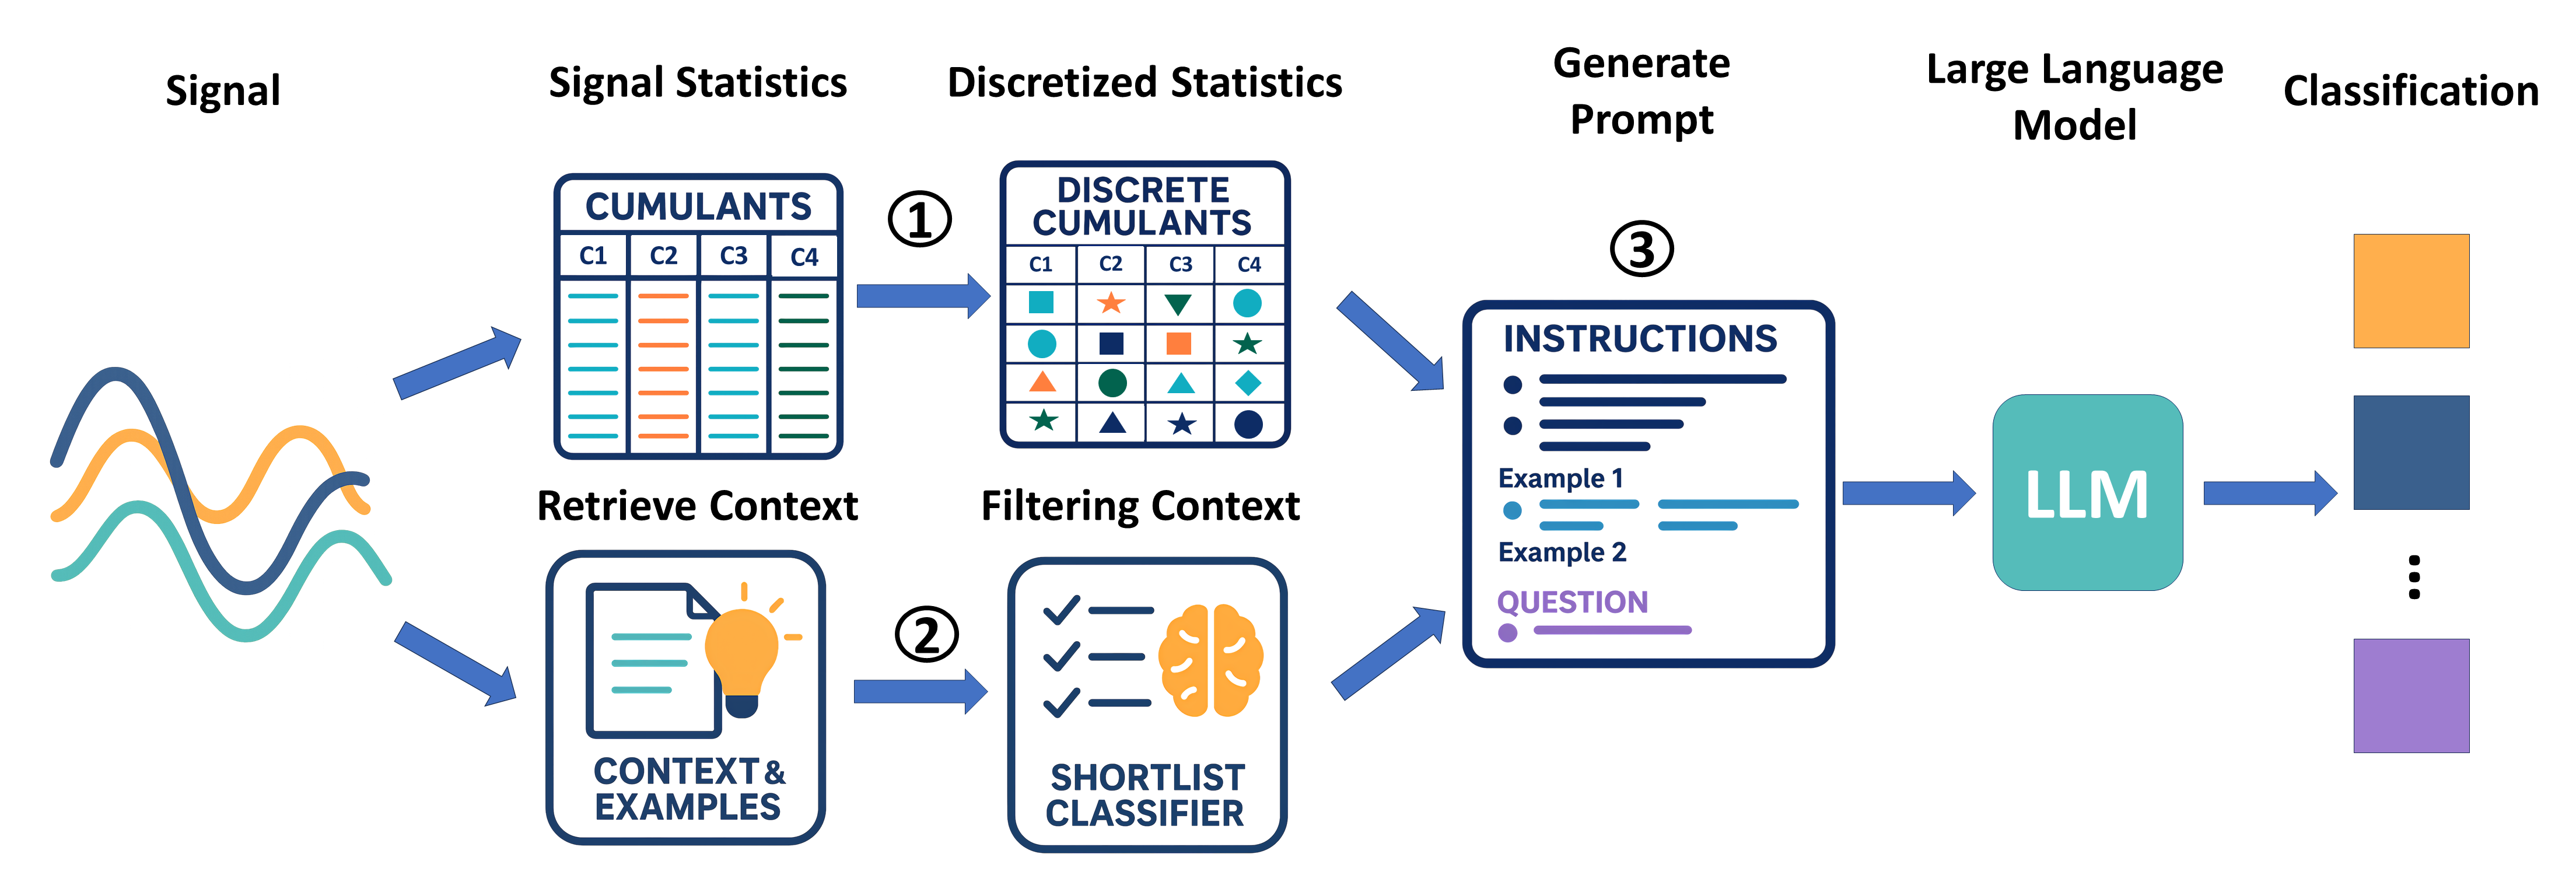
\includegraphics[width=0.9\textwidth]{FIGURES/disc/method.png}
\caption{Overview of the DiSC-AMC pipeline. (1) Raw I/Q signals are rendered as constellation diagrams and encoded into latent embeddings via a self-supervised visual encoder (DINOv2 ViT-B). (2) The continuous feature vector is quantized into ordinal bins and mapped to compact alphabetic symbols, achieving 3--5$\times$ token compression over raw floating-point serialization. (3) A two-stage retrieval module shortlists the $k_{\text{top}}$ most probable classes via centroid or FAISS proximity and retrieves the $k_{\mathrm{NN}}$ most similar labeled exemplars, forming a query-specific, pruned context. (4) The discretized query, retrieved exemplars, and candidate options are assembled into a $\sim$0.5K--1.3K token prompt. (5) A QLoRA fine-tuned DeepSeek-R1-Distill-Qwen-7B model performs chain-of-thought reasoning over the symbolic features before predicting the modulation class.}
\label{fig:disc_pipeline}
\end{figure*}

\subsection{Stage 1: Signal Representation and Feature Extraction}

DiSC-AMC supports two parallel feature extraction pathways. From the raw I/Q signal $x$, a \emph{statistical feature} vector is computed,
\begin{equation}
    s = \left[\hat\mu_2, \dots, \hat\mu_{10},\ \hat\kappa_1,\dots,\hat\kappa_4,\ \hat\gamma_1, \hat\gamma_2,\ \hat\sigma_{\kappa_1}, \hat\sigma_{\kappa_2},\ \mathrm{SNR}\right]^{\top} \in \mathbb{R}^{D_s},
\end{equation}
where $\hat\mu_k$ are sample central moments of order $k$, $\hat\kappa_j$ are $k$-statistics (minimum-variance unbiased cumulant estimators), $\hat\gamma_1,\hat\gamma_2$ are skewness and kurtosis, and SNR is the signal-to-noise ratio label provided with each sample (the generation SNR, not an estimate from the signal). Apart from this SNR label, which Plug-and-Play did not use, this is the statistical summary used earlier in this chapter (Section~\ref{sec:back}), with higher-order cumulants providing theoretical separation among BPSK, QPSK, and QAM families.

Alternatively, the signal is rendered as a constellation-diagram image and passed through a self-supervised visual \emph{encoder embedding} pathway: $z = g_\theta(\mathrm{img}(x)) \in \mathbb{R}^{D_z}$, reduced via PCA to $D_e \ll D_z$ components, $e = \mathrm{PCA}_{D_e}(z) \in \mathbb{R}^{D_e}$. This produces a compact, model-agnostic feature vector capturing learned visual patterns from the constellation geometry---the same DenoMAE-style representation philosophy developed in Chapter~\ref{chap:denomae}, here instantiated with a DINOv2 ViT-B encoder (frozen or fine-tuned depending on the scenario). Either feature vector ($s$ or $e$) is standardized via a \texttt{StandardScaler} fit on the training set.

\subsection{Stage 2: Discretization Mechanism}

The central innovation of DiSC-AMC maps any numerical signal representation to compact symbolic tokens, normalizing feature scales and compelling the model to focus on qualitative patterns rather than decimal precision. Given a feature vector $v \in \mathbb{R}^D$ (either $s$ or $e$), each dimension $v_j$ is independently quantized into one of $B$ ordinal bins via a \texttt{KBinsDiscretizer} with uniform strategy,
\begin{equation}
    q_j = \left\lfloor \frac{v_j - v_j^{\min}}{v_j^{\max} - v_j^{\min}} \cdot B \right\rfloor, \qquad q_j \in \{0, 1, \dots, B-1\},
\end{equation}
with bin edges fit on training data and applied deterministically at test time. Each integer bin index $q_j$ is encoded as a base-26 alphabetic symbol, $\phi(q_j) = \mathrm{base26}(q_j) \in \{A, B, \dots, Z, AA, \dots\}$, so the full signal representation becomes a sequence of symbolic tokens,
\begin{equation}
    f_{\mathrm{disc}}(v) = \left[\mathrm{feat}_1\!:\!\phi(q_1),\ \mathrm{feat}_2\!:\!\phi(q_2),\ \dots,\ \mathrm{feat}_D\!:\!\phi(q_D)\right].
\end{equation}
Discretization offers three benefits: (i) it compresses each feature from a multi-digit floating-point string to one or two characters, cutting prompt token count by roughly $3$--$5\times$; (ii) it abstracts away measurement noise, making the representation robust to small perturbations; and (iii) ordinal letter codes align naturally with the symbolic reasoning strengths of LLMs, rather than their comparatively weak numerical precision.

\subsection{Stage 3: Dynamic Context Construction}

Rather than a large, fixed exemplar set as in Plug-and-Play, DiSC-AMC builds a compact, query-specific context via two retrieval mechanisms, both driven by the self-supervised visual encoder.

\textbf{Context (few-shot) retrieval.} A FAISS index~\cite{faiss_douze2025} is built over the scaled feature vectors of all training signals. At inference, for a query feature vector $v_q$, the $k_{\mathrm{NN}}$ nearest training signals are retrieved via inverse-squared-distance weighting, grouped by class label, and added to the prompt as signal-specific, diverse few-shot demonstrations. When a minimum-class-diversity constraint is specified, the search radius expands (up to $3k_{\mathrm{NN}}$ candidates) with per-class brute-force scans to fill any missing classes.

\textbf{Candidate retrieval.} To further constrain the LLM's decision space, the full label set $\mathcal{M}$ is narrowed to the $k_{\mathrm{top}}$ most plausible classes using the same encoder, via one of four interchangeable strategies: (a) \emph{Centroid}---Euclidean distance from $z$ to per-class prototype centroids; (b) \emph{FAISS $k$NN}---inverse-distance-weighted voting among nearest neighbors; (c) \emph{DNN head}---softmax probabilities from a trained classification head; (d) \emph{Random Forest}---class vote counts from an RF classifier on encoder features. Applied to constellation images of the 10-class synthetic benchmark, candidate retrieval at $k_{\mathrm{top}}=5$ achieves \textbf{99.83\% recall}---the correct class is included in the shortlist in nearly every query---reducing the LLM's task from $C$-way to $k_{\mathrm{top}}$-way classification and preventing hallucinated out-of-vocabulary labels. Shortlist recall is an upper bound on final accuracy, not an accuracy figure itself: writing $R=\Pr(y\in\mathcal{C}(x))$ for recall, final accuracy satisfies $A = R\cdot\Pr(\hat y = y \mid y \in \mathcal{C}(x)) \leq R$. A 99.83\% shortlist recall therefore only bounds the opportunity available to the downstream LLM decision; it does not by itself guarantee, or report, how often that decision is correct.

\subsection{Stage 4: LLM Inference and Prompt Design}

The final prompt assembles three components: (1) an \emph{instruction template} (role description and response-format guide, optionally annotated with the candidate-retrieval method and feature type); (2) \emph{few-shot context} (the dynamically retrieved exemplars, each a discretized feature string paired with its ground-truth label); and (3) the \emph{query} (the discretized feature string of the test signal, followed by its candidate class options). The LLM is instructed to reason step-by-step inside \texttt{<think>} tags before outputting a single label, encouraging chain-of-thought deliberation over the symbolic features rather than the raw query.

\subsection{Experimental Setup}
\label{sec:disc_exp_setup}

\textbf{Datasets.} \emph{SynthMod-10} follows the Plug-and-Play generation protocol (Section~\ref{sec:exp}): 10 digital modulation classes (4ASK, 4PAM, 8ASK, 16PAM, CPFSK, DQPSK, GFSK, GMSK, OOK, OQPSK), 10,000 training signals, 200 in-distribution test queries ($-10$ to $+10$ dB), and 200 out-of-distribution (OOD) queries ($-15$ to $-11$ dB, never seen in training). \emph{RadioML 2018.01a}~\cite{oshea2018radioml} is a 24-class benchmark with real channel impairments (Rician fading, AWGN, frequency/phase drift), entirely disjoint from SynthMod-10, evaluated at five SNR levels ($-20,-10,0,+10,+20$ dB) with 2{,}400 training and 240 test samples per SNR level.

\textbf{Baselines.} Training-free baselines use the Plug-and-Play prompt format on DeepSeek-R1-Distill-Qwen (7B/32B); supervised/OOD baselines use DenoMAE~\cite{faysal2025denomae}, DenoMAE2.0~\cite{faysal2025denomae20improvingdenoisingmasked}, and NMformer~\cite{faysal2024nmformer} as fixed, non-LLM classification heads.

\textbf{Default configuration.} Unless noted otherwise, results use DeepSeek-R1-Distill-Qwen-7B fine-tuned via QLoRA on the training set, 5 discretization bins, FAISS $k_{\mathrm{NN}}=10$ context retrieval, and $k_{\mathrm{top}}=5$ candidate retrieval (FAISS voting over the $k=50$ nearest training signals) over DINOv2 encoder embeddings.

\textbf{Evaluation protocol.} Five scenarios isolate specific capabilities: (I) in-distribution classification on SynthMod-10; (II) near-OOD robustness on SynthMod-10; (III) cross-dataset transfer to RadioML with a fine-tuned encoder; (IV) cross-dataset transfer to RadioML with an unadapted encoder; (V) token and parameter efficiency. Ablations then dissect pipeline architecture choices and prompt-design tradeoffs.

\subsection{Results}
\label{sec:disc_results}

\textbf{Scenario I: In-distribution classification.} Table~\ref{tab:disc_scenario1} compares DiSC-AMC against supervised baselines on SynthMod-10. DiSC-AMC, using a 7B open-weight LLM with FAISS-retrieved exemplars over DINOv2 embeddings, achieves \textbf{83.00\%}, numerically above every supervised baseline including DenoMAE2.0 (82.40\%, the strongest encoder-only method from Chapter~\ref{chap:denomae}). This margin should be read descriptively rather than as an established statistical superiority: the test set is 200 queries, a binomial 95\% confidence half-width at this accuracy and sample size is approximately 5 points, and no repeated-seed or matched-split uncertainty estimate was computed for either row. The 0.6-point gap over DenoMAE2.0 is well within that uncertainty band; the result supports ``DiSC-AMC is competitive with the strongest supervised baseline,'' not ``DiSC-AMC is proven superior to it.''

\begin{table}[htbp]
\centering
\caption{Scenario I: In-distribution classification on SynthMod-10.}
\label{tab:disc_scenario1}
\begin{tabular}{lcc}
\toprule
Model & Params & Acc.\ (\%) \\
\midrule
DINOv2 & 86M & 65.33 \\
NMformer~\cite{faysal2024nmformer} & 86M & 71.60 \\
ViT~\cite{faysal2025denomae20improvingdenoisingmasked} & 86M & 79.90 \\
DEiT~\cite{faysal2025denomae20improvingdenoisingmasked} & 86M & 81.20 \\
MoCov3~\cite{faysal2025denomae20improvingdenoisingmasked} & 86M & 81.00 \\
BEiT~\cite{faysal2025denomae20improvingdenoisingmasked} & 86M & 80.40 \\
MAE~\cite{faysal2025denomae20improvingdenoisingmasked} & 86M & 80.10 \\
DenoMAE~\cite{faysal2025denomae} & 86M & 81.30 \\
DenoMAE2.0~\cite{faysal2025denomae20improvingdenoisingmasked} & 86M & 82.40 \\
\textbf{DiSC-AMC (ours)} & \textbf{7B} & \textbf{83.00} \\
\bottomrule
\end{tabular}
\end{table}

\textbf{Scenario II: Near-OOD robustness.} Shifting the test set to an unseen SNR range ($-15$ to $-11$ dB) outside the training distribution, DiSC-AMC maintains \textbf{82.50\%} OOD accuracy (Table~\ref{tab:disc_scenario2}), a drop of only 0.5 points from in-distribution, far exceeding standalone encoder baselines.

\begin{table}[htbp]
\centering
\caption{Scenario II: Near-OOD robustness on SynthMod-10.}
\label{tab:disc_scenario2}
\begin{tabular}{lcc}
\toprule
Model & Params & OOD Acc.\ (\%) \\
\midrule
DINOv2 & 86M & 63.90 \\
DenoMAE2.0~\cite{faysal2025denomae20improvingdenoisingmasked} & 86M & 63.25 \\
\textbf{DiSC-AMC (ours)} & \textbf{7B} & \textbf{82.50} \\
\bottomrule
\end{tabular}
\end{table}

\textbf{Scenarios III \& IV: Cross-dataset transfer to RadioML.} These scenarios test whether DiSC-AMC's reasoning amplifies an encoder backbone's own classification head when transferred to the entirely disjoint 24-class RadioML benchmark, with the encoder either fine-tuned (III) or left unadapted (IV). In both scenarios, the classification head and, in Scenario III, the encoder backbone are trained on RadioML's own 12,000 labeled training samples (Section~\ref{sec:disc_exp_setup}); this is \emph{supervised target-domain adaptation}, not label-free transfer---RadioML labels are used in both scenarios, and the distinction between them is whether the encoder's weights are updated (III) or held fixed while only a head is fit (IV), not whether target labels are used at all. With this scoping, Table~\ref{tab:disc_scenario3} shows that with a fine-tuned DINOv2 backbone, DiSC-AMC reaches \textbf{76.25\%} at $+20$ dB versus just 9.58\% for the fine-tuned encoder's own head---an \textbf{8$\times$} improvement. Table~\ref{tab:disc_scenario4} shows the same effect holds with the encoder weights left unadapted (only the head is trained on RadioML labels): DiSC-AMC with an unadapted DINOv2 reaches 45.42\% at $+20$ dB versus 7.08\% for the head alone. In both scenarios, standalone encoder heads plateau below 15\% across all SNR levels, confirming that reasoning---not the encoder alone---drives cross-dataset generalization. Notably, DenoMAE2.0 as the DiSC-AMC backbone \emph{underperforms} DINOv2 on RadioML at higher SNRs (Table~\ref{tab:disc_scenario3}, $+10$/$+20$ dB), indicating that DenoMAE2.0's synthetic-data-trained features do not retrieve informative neighbors on this out-of-family dataset even though they excel in-distribution (Scenario I).

\begin{table}[htbp]
\centering
\caption{Scenario III: Cross-dataset transfer with a fine-tuned encoder (RadioML 2018.01a, 24 classes).}
\label{tab:disc_scenario3}
\begin{tabular}{c cc cc}
\toprule
 & \multicolumn{2}{c}{Fine-tuned encoder (\%)} & \multicolumn{2}{c}{DiSC-AMC (\%)} \\
SNR (dB) & DINOv2 & DenoMAE2.0 & DINOv2 & DenoMAE2.0 \\
\midrule
$-20$ & 3.33 & 4.17  & 19.58 & 17.92 \\
$-10$ & 3.33 & 5.42  & 17.50 & 19.17 \\
$0$   & 6.67 & 8.75  & 40.83 & 25.00 \\
$+10$ & 8.75 & 13.33 & 72.50 & 24.17 \\
$+20$ & 9.58 & 11.25 & \textbf{76.25} & 21.25 \\
\bottomrule
\end{tabular}
\end{table}

\begin{table}[htbp]
\centering
\caption{Scenario IV: Cross-dataset transfer with an unadapted encoder (RadioML 2018.01a, 24 classes).}
\label{tab:disc_scenario4}
\begin{tabular}{c cc cc}
\toprule
 & \multicolumn{2}{c}{Encoder only (\%)} & \multicolumn{2}{c}{DiSC-AMC (\%)} \\
SNR (dB) & DINOv2 & DenoMAE2.0 & DINOv2 & DenoMAE2.0 \\
\midrule
$-20$ & 3.75  & 3.33  & 10.83 & 15.42 \\
$-10$ & 5.00  & 2.92  & 11.67 & 5.83 \\
$0$   & 6.67  & 9.58  & 28.33 & 12.50 \\
$+10$ & 15.00 & 14.58 & 36.25 & 5.83 \\
$+20$ & 7.08  & 12.92 & \textbf{45.42} & 6.25 \\
\bottomrule
\end{tabular}
\end{table}

\textbf{Scenario V: Token and parameter efficiency.} Table~\ref{tab:disc_scenario5} isolates the cost of reasoning. The Plug-and-Play baseline requires a 2.9K-token prompt and reaches only 5.20\% on a 7B model; even the proprietary o3-mini reaches 69.92\%. DiSC-AMC's training-free 7B model, without retrieved context exemplars, reaches \textbf{71.9\%} valid-output accuracy (143 of 199 valid answers; 71.5\% over all 200 queries) at just \textbf{0.5K tokens}---surpassing the proprietary o3-mini baseline at roughly one-sixth the prompt length.
% TODO(author-audit): o3-mini 69.92% is all-query accuracy over 3 passes of 332 prompts (presentation/Results - 08_01_25.xlsx; 695/994), not the 200-query test set; consider stating this protocol difference.

\begin{table}[htbp]
\centering
\caption[Scenario V: Token and parameter efficiency.]{Scenario V: Token and parameter efficiency. Parameter counts of proprietary models are not publicly disclosed.}
\label{tab:disc_scenario5}
\begin{tabular}{lccc}
\toprule
Model & Params & \#Tokens & Acc.\ (\%) \\
\midrule
DeepSeek-R1 (PnP) & 7B & 2.9K & 5.20 \\
DeepSeek-R1 (PnP) & 32B & 2.9K & 47.80 \\
o3-mini (PnP) & -- & 2.9K & 69.92 \\
\textbf{DeepSeek-R1 (DiSC-AMC, training-free)} & \textbf{7B} & \textbf{0.5K} & \textbf{71.9} \\
\bottomrule
\end{tabular}
\end{table}

\subsection{Ablation Studies}
\label{sec:disc_ablations}

Using DeepSeek-R1-Distill-Qwen-7B and GLM-4.6V-Flash in a training-free setting, four independent design axes are varied: candidate-retrieval strategy, feature representation, context retrieval (RAG), and distribution shift.

\textbf{Candidate retrieval: FAISS vs.\ centroid.} FAISS $k$NN retrieval substantially outperforms centroid-based selection: 66.1\% vs.\ 32.8\% in-distribution, and 62.6\% vs.\ 42.5\% under moderate OOD shift. Centroid-selected exemplars cluster around class means and lack query-specific diversity; a key factor is \emph{SNR matching}---because signal statistics vary substantially with SNR, exemplars from a mismatched noise level confuse rather than guide the LLM, and FAISS retrieval naturally preserves SNR proximity where centroid selection does not.

\textbf{Feature representation: embeddings vs.\ statistics.} Replacing discretized statistics with self-supervised encoder embeddings as the retrieval feature consistently improves accuracy: the best embedding-based configuration reaches 71.5\% in-distribution versus 69.0\% for the best statistics-only configuration---the encoder captures visual invariances of constellation diagrams that cumulant statistics do not.

\textbf{Context retrieval (RAG) vs.\ fixed exemplars.} RAG-augmented and fixed-exemplar pipelines achieve comparable mean accuracy in-distribution (47.2\% vs.\ 51.8\%); RAG's dynamic retrieval catches up to the fixed set at 52.6\% under OOD shift, indicating that \emph{which} exemplars are retrieved (FAISS vs.\ centroid) matters far more than \emph{how many} are added per query.

\textbf{Out-of-distribution generalization and the noise floor.} Accuracy degrades gracefully under moderate OOD shift ($-11$ to $-15$ dB): the best FAISS configuration retains 68.5\%, only 3 points below its 71.5\% in-distribution score. Under extreme shift ($-30$ dB), however, all configurations collapse to near-random levels ($\sim$5--10\%)---at this noise level constellation diagrams become effectively featureless, so the self-supervised encoder's embeddings lose discriminative structure and both retrieval and classification degrade to chance. This is a fundamental limitation of any retrieval pipeline built on visual signal representations, and directly echoes the low-SNR collapse observed for DenoMAE in Chapter~\ref{chap:denomae}.

\textbf{Prompt design tradeoffs.} Table~\ref{tab:disc_prompt_format} isolates prompt format in the training-free setting. The 7B DeepSeek model under the raw Plug-and-Play prompt achieves only 9\%, confirming that floating-point serialization overwhelms small models; Gemini-2.5-Flash with a 1.3K-token DiSC-AMC prompt reaches 45.5\%, exceeding a 32B DeepSeek PnP + candidates baseline (32.5\%) at under half the token cost, and Gemini-2.5-Pro at 0.9K tokens reaches 51.0\%---the best configuration in this table. Increasing the candidate-set size $k_{\mathrm{top}}$ from 4 to 5 yields a marginal gain (44.5\%$\to$45.5\%) for a small token cost; expanding to $k_{\mathrm{top}}=10$ (10 bins) expands the prompt to 2.9K tokens while accuracy \emph{drops} to 29.5\%, since candidate-retrieval recall already reaches 99.83\% at $k_{\mathrm{top}}=5$. Discretization granularity shows a similar ``less is more'' pattern: Gemini-2.5-Flash peaks at 5 bins (45.5\%) and degrades monotonically with finer bins, while the more capable Gemini-2.5-Pro peaks later, at 10 bins (47.5\%), before declining---coarse symbolic codes align better with LLM reasoning over noisy physical-layer signals than high-precision numerical detail, for most models.

\begin{table}[htbp]
\centering
\caption[Effect of prompt format on training-free LLMs (centroid candidate retrieval, no RAG).]{Effect of prompt format on training-free LLMs (centroid candidate retrieval, no RAG). Parameter counts of proprietary models are not publicly disclosed.}
\label{tab:disc_prompt_format}
\begin{tabular}{llccc}
\toprule
Method & Model & Params & \#Tokens & Acc.\ (\%) \\
\midrule
PnP & DeepSeek-R1 & 7B & 2.9K & 5.20 \\
PnP & DeepSeek-R1 & 32B & 2.9K & 47.80 \\
PnP & o3-mini & -- & 2.9K & 69.92 \\
PnP + candidates & DeepSeek-R1 & 7B & 2.9K & 9.00 \\
PnP + candidates & DeepSeek-R1 & 32B & 2.9K & 32.50 \\
PnP + candidates & Gemini-2.5-Flash & -- & 2.9K & 29.50 \\
PnP + candidates & Gemini-2.5-Pro & -- & 2.9K & 42.50 \\
\textbf{DiSC-AMC} & DeepSeek-R1 & 7B & 1.3K & 33.50 \\
\textbf{DiSC-AMC} & DeepSeek-R1 & 32B & 1.3K & 39.00 \\
\textbf{DiSC-AMC} & Gemini-2.5-Flash & -- & 1.3K & 45.50 \\
\textbf{DiSC-AMC} & Gemini-2.5-Pro & -- & 0.9K & \textbf{51.00} \\
\bottomrule
\end{tabular}
\end{table}

\subsection{RQ1 Meets RQ2: Does the Encoder Matter?}
\label{sec:rq1_meets_rq2}

Scenarios III and IV (Tables~\ref{tab:disc_scenario3}--\ref{tab:disc_scenario4}) are deliberately designed to probe the seam between RQ1 (representation) and RQ2 (reasoning): DiSC-AMC's retrieval stage depends entirely on an RQ1 encoder, so its RadioML performance is a direct test of whether reasoning can compensate for representation quality, or whether it is bottlenecked by it.

With a \emph{fine-tuned} DINOv2 backbone, DiSC-AMC reaches 76.3\% at $+20$ dB versus 9.6\% for the DINOv2 head alone---a $\mathbf{8\times}$ improvement from reasoning over the same features. Strikingly, this amplification holds even with an \emph{unadapted} DINOv2 encoder, where only the classification head was trained: DiSC-AMC still reaches 45.4\% versus 7.1\% for the head alone, a $\mathbf{6\times}$ gain, showing that reasoning amplifies a general-purpose visual encoder without any target-domain fine-tuning, provided its embeddings carry some class-relevant structure.

The counter-case is equally informative. With DenoMAE2.0 as the backbone---the stronger encoder on SynthMod-10 (82.4\% vs.\ DINOv2's 65.3\%, Table~\ref{tab:disc_scenario1})---DiSC-AMC plateaus at or below 25\% across every SNR on RadioML (Table~\ref{tab:disc_scenario3}), and in the unadapted setting its own head alone \emph{beats} DiSC-AMC at $+10$ and $+20$ dB (Table~\ref{tab:disc_scenario4}): reasoning provides no gain, and can even be outperformed by the plain head. The difference is not reasoning capacity but retrieval quality: DenoMAE2.0 was trained exclusively on the synthetic SynthMod-10 distribution, so its nearest neighbors on the out-of-family RadioML dataset are not meaningfully related to the query's true class, and the LLM is reasoning over uninformative context. DINOv2, pretrained on broad natural-image self-supervision rather than narrow synthetic constellations, retrieves more generically relevant neighbors even without wireless-specific adaptation.

\textbf{Difficult finding:} reasoning only helps when the encoder's nearest neighbors are meaningful. This is the dissertation's clearest demonstration that RQ2's gains are conditional on RQ1: DiSC-AMC is not an encoder-agnostic amplifier, but a mechanism that converts representation quality into classification accuracy, and inherits representation failures just as readily as it inherits representation strengths.

\subsection{Testing a Non-Generative Classifier: Jev}
\label{sec:jev}

The DiSC-AMC pipeline was designed around chain-of-thought generation: the LLM reasons inside \texttt{<think>} tags before committing to a label. A natural question is whether the same discretized, retrieval-augmented prompt transfers to a fundamentally different decision mechanism---a non-generative classifier that scores a fixed set of options rather than generating free text. We tested this using \textbf{Jev}, which consumes three inputs---a \emph{state} (the full DiSC-AMC prompt: role, binned statistics, retrieved exemplars, and the query), a set of \emph{options} (the $k_{\mathrm{top}}$ shortlisted candidate classes), and \emph{criteria} (one fixed natural-language description per option, e.g., for 16QAM: ``16 symbols on a 4$\times$4 square grid, varying both amplitude and phase'')---and returns a single selected option with a probability, with no reasoning trace.

Table~\ref{tab:jev_results} compares Jev against the paper's generative LLMs (Gemini-2.5-Pro on the Table~\ref{tab:disc_prompt_format} prompt; DeepSeek-R1-Distill-Qwen-7B on RadioML) under three identical shortlist conditions.

\begin{table}[htbp]
\centering
\caption{Jev vs.\ the paper's generative LLM on identical shortlists and candidate sets.}
\label{tab:jev_results}
\begin{tabular}{lccc}
\toprule
Condition & Paper LLM & Jev (default) & Jev (tailored) \\
\midrule
Centroid shortlist, 10 classes & 51.0\% & 53.5\% & 56.5\% \\
FAISS shortlist, 10 classes & 71.5\% & 65.0\% & 65.0\% \\
RadioML $+20$ dB, 24 classes & 76.3\% & 33.3\% & 32.5\% \\
\bottomrule
\end{tabular}
\end{table}

On the centroid-shortlist condition, Jev modestly \emph{outperforms} Gemini-2.5-Pro on the identical Table~\ref{tab:disc_prompt_format} prompt (56.5\% tailored vs.\ 51.0\%, a $+5.5$-point gain), showing the DiSC-AMC prompt format transfers to a non-generative scoring mechanism. On the FAISS-shortlist condition the two are closer (65.0\% vs.\ 71.5\%). But on RadioML, where 13 of the 24 classes differ only in modulation \emph{order} (e.g., 16/32/64QAM, several APSK variants), Jev collapses to 32.5\textendash33.3\% while the reasoning LLM reaches 76.3\%---more than double. \textbf{Finding:} the DiSC prompt transfers to a non-generative model for coarse class discrimination, but fine-grained order discrimination, which requires reasoning about relative structure rather than matching a fixed description, needs a model that can actually reason over the symbolic evidence rather than score against static criteria.

This comparison, however, is not a clean controlled experiment, and the limitations are reported explicitly rather than left implicit in the headline numbers:
\begin{itemize}
    \item \textbf{Prompt not designed for Jev:} tailoring only removed the \texttt{<think>}-tag and output-format instructions meant for generative decoding; no Jev-specific prompt was searched for.
    \item \textbf{Criteria cannot carry query-specific evidence:} a fixed per-class blurb (e.g., restating that 16QAM, 32QAM, and 64QAM differ only in symbol count) cannot encode the query's actual discretized statistics, which live only in the state.
    \item \textbf{Default runs had empty criteria:} a configuration bug sent null descriptions in the untailored condition, so those runs saw class names only, not even the static blurbs.
    \item \textbf{Two changes confounded at once:} the tailored condition simultaneously strips the generative-decoding rules and adds criteria, so their separate contributions are not isolated.
    \item \textbf{Small, single runs:} each condition used 200--240 queries, one trial, one model version; tailoring moved results by $-1.5$ to $+3.0$ points (roughly 6 queries)---within the noise floor of a single run at this sample size.
    \item \textbf{Options are pre-filtered by the shortlist:} a class the candidate-retrieval shortlist drops is never available to Jev; 31\% of plain-FAISS-shortlisted queries had only one option, trivializing the decision for those queries.
\end{itemize}

\textbf{Takeaway:} the DiSC-AMC prompt format is not tied to generative decoding, but a fair comparison between reasoning and non-reasoning classifiers on this task requires query-specific criteria and repeated runs at larger sample sizes---work left open in Section~\ref{sec:future_work}.

\subsection{Qualitative Reasoning: Grounded Inference and Confident Confabulation}
\label{sec:qualitative_reasoning}

Aggregate accuracy numbers obscure \emph{how} the fine-tuned model reaches its answers. Inspecting individual chain-of-thought traces reveals that the 83\% fine-tuned model's correct and incorrect predictions differ qualitatively, not just in outcome.

On a correctly classified 8ASK query (true label 8ASK, options \{8ASK, 4PAM, 4ASK\}, 5.73 dB), the model grounds its answer in a specific, checkable feature-to-hypothesis link: ``The feature pc\_0 is E, which is the highest bin. The rest of the features (pc\_1 to pc\_9) are mostly C and D. [\ldots] For 8ASK, we'd expect a wider range of amplitude values, leading to more varied bins. [\ldots] For 4PAM, there are only four amplitude levels, so the features should reflect a more limited range.'' This reasoning ties the spread of the binned features directly to the number of amplitude levels each candidate modulation implies---a correct and verifiable inference.

On an incorrectly classified query (true label CPFSK, predicted GFSK, options \{GFSK, CPFSK\}, $-2.70$ dB), the model's own trace admits the features are uninformative, then answers anyway: ``GFSK (Gaussian Filtered-Smoothed FM) [\ldots] CPFSK (Chirp-Frequency-Smoothed Keyed FM) [\ldots] I notice that the features don't strongly indicate a particular scheme. [\ldots] Given the options and the features, the most probable classification is GFSK.'' Both expansions are also wrong (GFSK is Gaussian \emph{Frequency} Shift Keying; CPFSK is \emph{Continuous}-Phase FSK), suggesting the model's uncertainty is genuine but its explanation does not surface that uncertainty to a reader---it produces a confident-sounding rationale around what amounts to a guess. \textbf{Finding:} even the strongest (83\%) configuration fails on the hardest class pair in the benchmark, two continuous-phase FSK variants that are physically similar, and its failure mode is not an obviously garbled trace but a fluent one built on an incorrect premise.

Comparing the fine-tuned (83.0\%) and training-free (71.0\%) configurations on identical retrieval---same FAISS shortlist, same DINOv2 embeddings, same 10 retrieved exemplars, same 5 bins, differing only in whether QLoRA fine-tuning was applied (166 vs.\ 142 of 200 correct)---shows the same pattern at smaller scale. A correct training-free prediction (true and predicted GFSK, 1.99 dB) reasons from one weak but ultimately correct heuristic after dismissing the rest: ``The other features don't clearly point towards one over the other, but the SNR is a strong indicator. Therefore, I'm leaning towards GFSK.'' An incorrect training-free prediction (true GFSK, predicted CPFSK, $-6.85$ dB) again builds a plausible-sounding cumulant argument on an incorrect premise: ``GFSK is Gaussian Filtered SSB Modulation. [\ldots] I'm leaning towards CPFSK because I remember that CPFSK signals have non-zero even-order cumulants''---GFSK is frequency-shift keying, not single-sideband modulation. Fine-tuning does not change the \emph{style} of reasoning observed in these traces; it changes how often the underlying domain knowledge the model draws on is correct, which is consistent with QLoRA correcting factual associations (e.g., modulation-family definitions) rather than altering the reasoning strategy itself.

These qualitative traces temper the chapter's quantitative claims: DiSC-AMC's interpretability advantage over end-to-end classifiers is real---every prediction ships with an inspectable rationale---but that rationale is not a reliable confidence signal. A fluent explanation can accompany a wrong answer as readily as a right one, which matters for any deployment that would use the chain-of-thought text itself (rather than just the final label) to decide how much to trust a given classification.

\subsection{Discussion: Answering RQ2}
\label{sec:disc_discussion}

DiSC-AMC provides the dissertation's strongest evidence for Research Question 2 (RQ2): \textit{Can RF statistics and relevant examples be given to an LLM efficiently enough for useful, open-set AMC?} Two complementary results support a confident \textbf{yes, within bounds}. First, a QLoRA fine-tuned 7B model reaches 83.00\% in-distribution and 82.50\% OOD accuracy on SynthMod-10, matching or surpassing every supervised baseline evaluated, including DenoMAE2.0---demonstrating that symbolic, retrieval-augmented reasoning is not merely a cheaper substitute for supervised classification but can be competitive with it. Second, a training-free 7B model reaches 71.9\% accuracy at 0.5K tokens, exceeding the proprietary o3-mini model given 2.9K tokens of raw statistics (69.92\%)---demonstrating that \emph{prompt construction, not model scale, is the dominant driver of LLM-based AMC accuracy}.

The bounds on this answer come from three directions, each explored in the preceding subsections. On cross-dataset transfer to RadioML, DiSC-AMC amplifies a frozen or fine-tuned encoder's own head by up to 8$\times$ (Section~\ref{sec:rq1_meets_rq2}), but only when the encoder's nearest neighbors remain informative: DenoMAE2.0's synthetic-trained embeddings, which excel in-distribution, retrieve poorly on RadioML, so the composition's ceiling is ultimately set by the quality of the RQ1 representation it retrieves over (Chapter~\ref{chap:denomae}, Chapter~\ref{chap:cdrf})---reasoning cannot manufacture class signal an encoder's embeddings do not carry. On decision mechanism, the DiSC-AMC prompt transfers to a non-generative classifier (Jev) for coarse, well-separated classes, but a reasoning LLM is needed for fine-grained order discrimination on RadioML's APSK/QAM families (Section~\ref{sec:jev}). On interpretability, qualitative inspection (Section~\ref{sec:qualitative_reasoning}) shows that chain-of-thought explanations are fluent regardless of correctness, so the rationale text is not itself a reliable confidence signal, even from the best-performing configuration. The one hard noise limit is physical rather than algorithmic: below roughly $-30$ dB, constellation-based features of any kind collapse to chance, for both retrieval and final classification.

\textbf{Connection to the Dissertation Framework:} Together, Plug-and-Play and DiSC-AMC demonstrate that the \textit{intelligent reasoning engine} of this dissertation's modular framework can be built economically: training-free when deployment cost dominates, or lightly fine-tuned when accuracy must match dedicated supervised encoders---in both cases at a small fraction of the parameter count of frontier LLMs. This validates the dissertation's central thesis that wireless foundation-model capabilities need not be built through massive isolated training, but can be assembled by strategically integrating pre-trained vision (RQ1, Chapters~\ref{chap:denomae}--\ref{chap:cdrf}) and language (RQ2) world knowledge. DiSC-AMC's retrieval stage is itself a direct composition of RQ1 and RQ2: it is the self-supervised encoder from Chapter~\ref{chap:denomae} that supplies the exemplars the LLM reasons over, making DiSC-AMC the dissertation's concrete demonstration that the framework's components compose rather than merely coexist. Section~\ref{sec:wireless_meta_task} (Chapter~\ref{chap:meta_task}) returns to this composition from the RQ3 (adaptation) side, testing whether Meta-Task's learnable regularization can further improve the DiSC-AMC pipeline on RadioML.

Overall, this chapter represents a substantive step toward practical, open-set wireless reasoning with LLMs. The transition from Plug-and-Play to DiSC-AMC shows concretely how an initial proof-of-concept, once its cost bottleneck is diagnosed, can be redesigned into a deployment-realistic pipeline---while being explicit about where that pipeline's limits still lie.

\FloatBarrier

% Bibliography commands moved to main.tex to avoid conflicts
% \bibliographystyle{ieeetr}
% \bibliography{egbib}

